% !TEX root = ../thesis.tex
\chapter{Results and Discussion}
\label{chap:results}

We will first look at the web application results based on the user's feedback, and then we will look into the insights and potential feedback the NLP process could provide the user. We then also look to review the overall process. 

We will compare the web application's results against the comparative judgment, Elo ranking, and the score we created for the tweets on Twitter. With the insights of the NLP for feedback to the user, we will look at what insights got made. Additionally, we will look at if any of the knowledge extracted generated provides any meaningful feedback to the user.



\section{Tweet Ranking Results} 
\label{sec:reaults_ranking}

\begin{figure}[h]
	\centering
	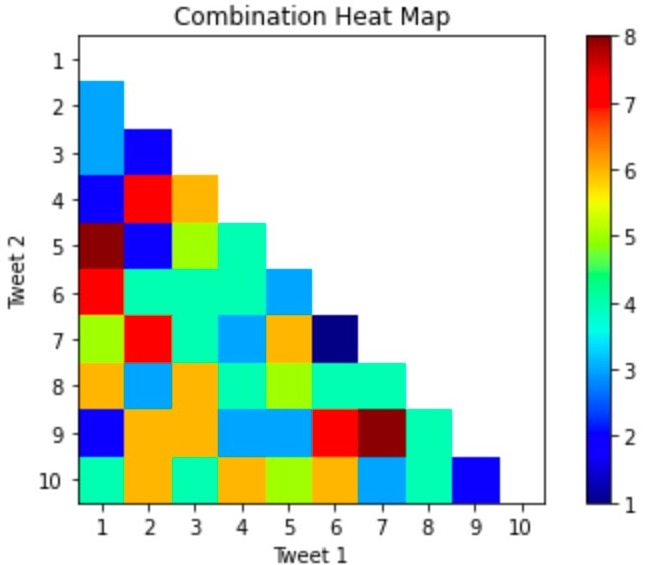
\includegraphics[width=7cm]{combination_heat_map.png}
	\caption{The web applicaitons generated results compared agaist each other.}
	\label{fig:combinations}
	
\end{figure}

\begin{figure}[h]
	\centering
	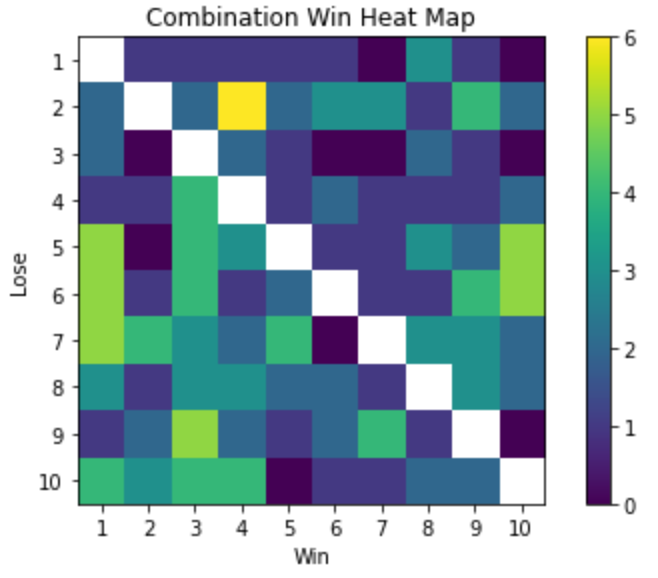
\includegraphics[width=7cm]{combination_win_heat_map.png}
	\caption{The web applicaitons generated results compared agaist each other.}
	\label{fig:combination_wins}
	
\end{figure}


While looking at fig \ref{fig:web_app_results}, we can see that the Elo and comparative judgement ranking generated very similar results. However, as we can see, the tweets coming in 6th, 7th and 8th a slight variation in the results.

\begin{figure}[h]
	\centering
	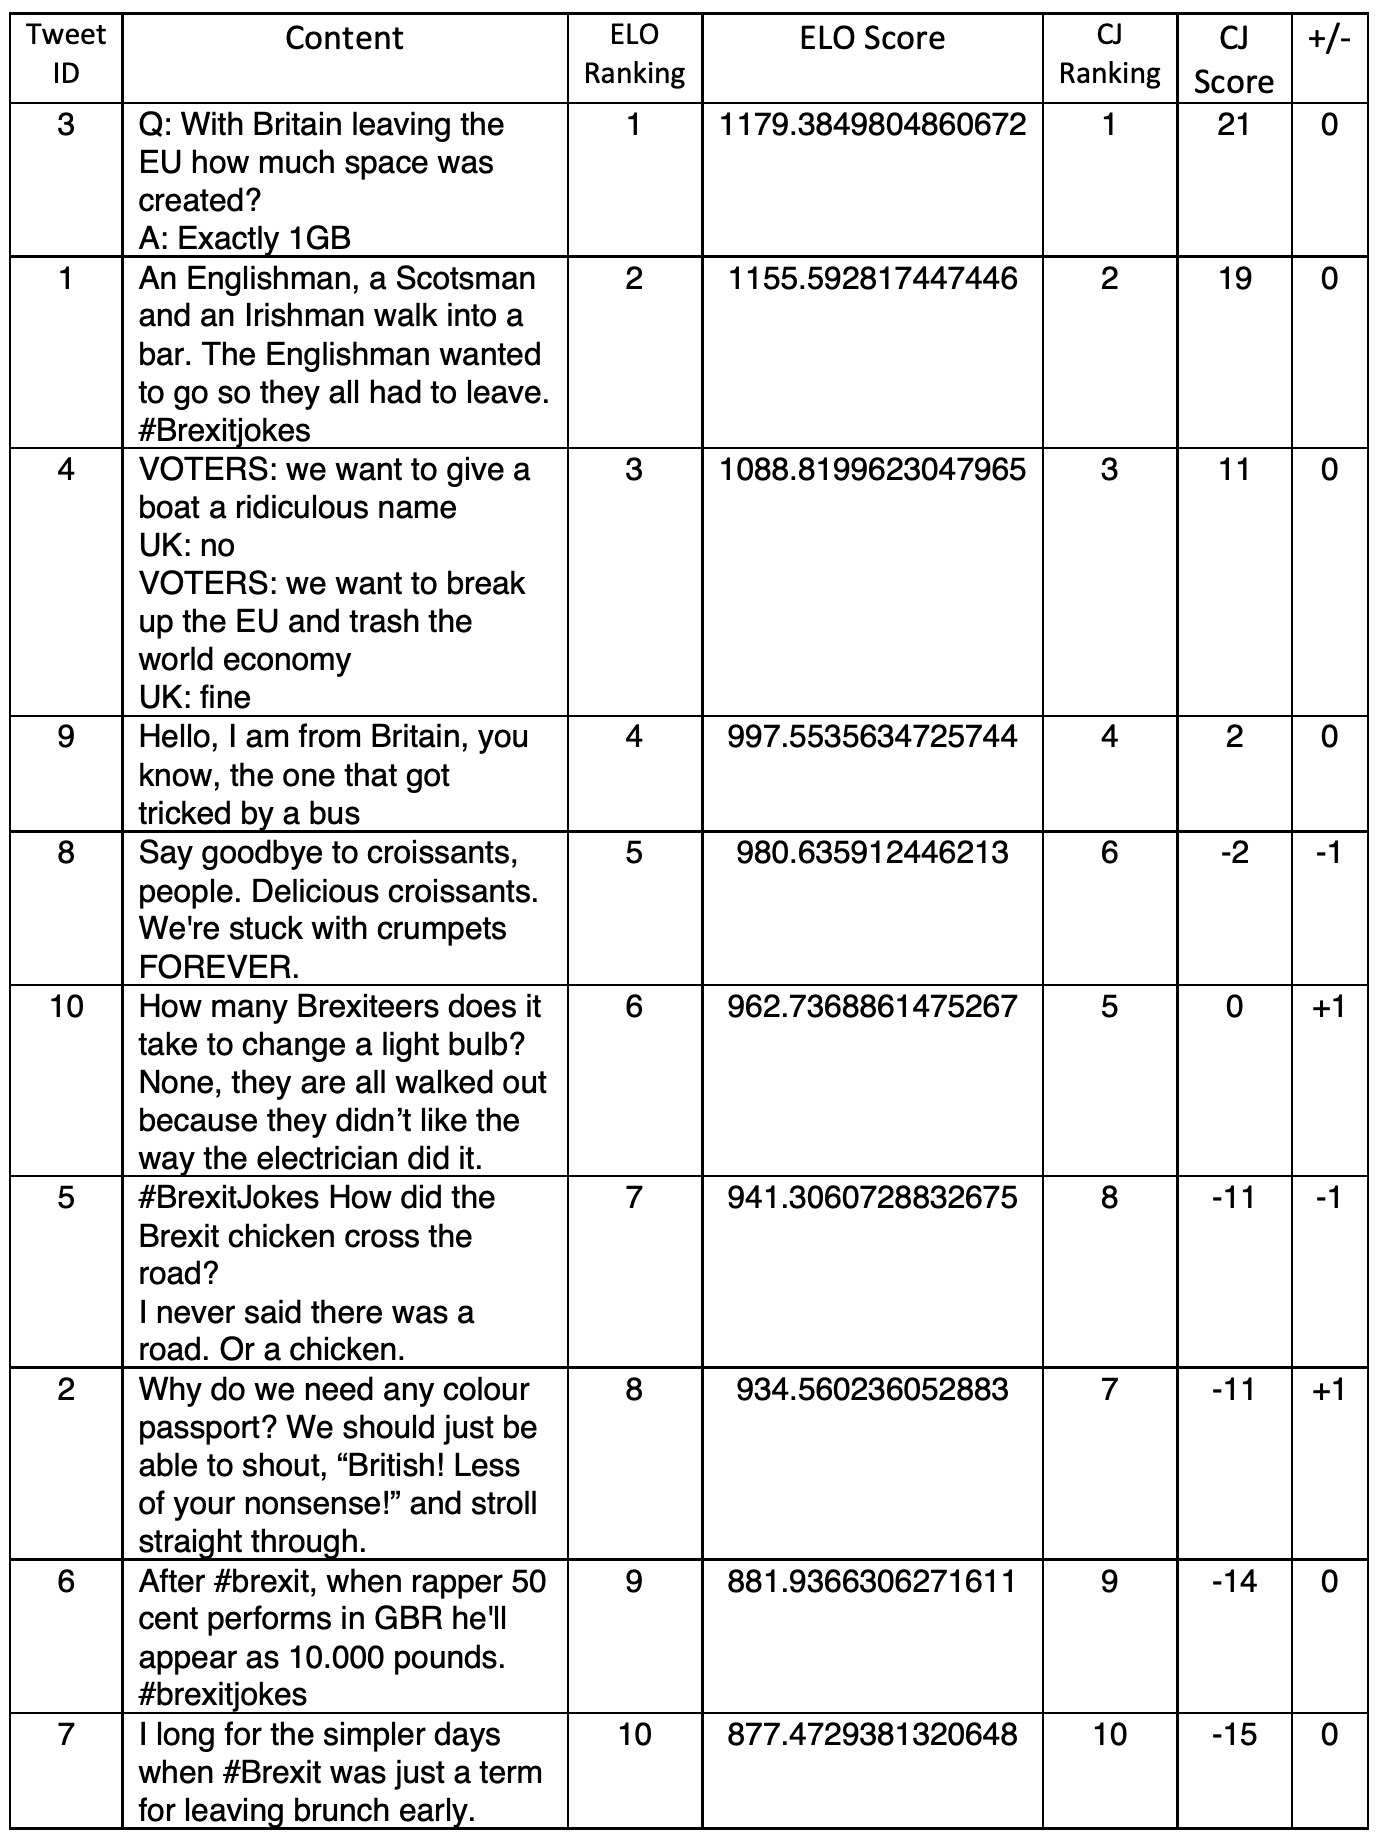
\includegraphics[width=10cm]{web_app_results.png}
	\caption{The web applicaitons generated results compared agaist each other.}
	\label{fig:web_app_results}
	
\end{figure}

\section{NLP Feedback and Insights}
\label{sec:reaults_NLP}

\section{Overall Results}
\label{sec:reaults_NLP}

